% SUI project
% Juraj Holub
% xholub40@stud.fit.vutbr.cz

\documentclass[a4paper, 11pt]{article}
\usepackage[utf8]{inputenc}
\usepackage[slovak]{babel}
\usepackage[left=1.5cm,top=2.5cm,text={18cm,25cm}]{geometry}
\usepackage[unicode]{hyperref}
\usepackage{amsmath, amsthm, amsfonts, amssymb}
\usepackage{dsfont}
\setlength{\parindent}{1em}
\usepackage{hyperref}
\usepackage{graphicx}
\usepackage{float}
\usepackage{wrapfig}
\usepackage{listings}
\usepackage{url}
\usepackage{cite}
\usepackage{multicol}
\usepackage{color}
\usepackage{multirow}
\usepackage{colortbl}
\usepackage[table,xcdraw]{xcolor}
\usepackage{pifont}
\usepackage{bm}
%\date{}

\lstset{
	basicstyle=\small\ttfamily,
}


\newcommand{\cmark}{\ding{51}}%
\newcommand{\xmark}{\ding{55}}%

\begin{document}
\begin{titlepage}
	\begin{center}
		\Huge
		\textsc{Fakulta informačních technologií \\
			Vysoké učení technické v~Brně} \\
		\vspace{\stretch{0.382}}
		{\LARGE
			SUI - Umělá inteligence a strojové učení \\ 
			\medskip 
			\Large{
				Umělá inteligence pro Válku kostek
			}
			\vspace{\stretch{0.618}}}
		\setlength{\parindent}{0.3em}\\
		{\Large 2021} \\
		{\Large Doležel Marek (xdolez67)} \\
		{\Large Holub Juraj (xholub40)} \\
		{\Large Mateáš Branislav (xmatea00)} \\
		{\Large Rádsetoulal Vlastimil (xradse00)}
	\end{center}
\end{titlepage}

\tableofcontents
\newpage

\section{Úvod}



\section{Prehľadávanie stavového priestoru}\label{sec:dfs}

Naša implementácia prehľadávania stavového priestoru je založená na algoritme \textit{Max-N};\footnote{\url{https://docplayer.net/131108557-Expectimax-n-a-modification-of-expectimax-algorithm-to-solve-multiplayer-stochastic-game.html}}. Algoritmus je vizualizovaný na obrázku~\ref{img:dfs}. Hranaté uzly označujú prvý ťah každého hráča v aktuálnom kole (hráči P1, P2, P3 a P4). Aktuálny hráč na ťahu určí nasledujúce možné ťahy. Avšak v našej hre počas jedného kola môže hráč podľa pravidiel urobiť viacero ťahov. Preto sa každý hráčov ťah expanduje ďalej až do úrovne $n$, kde $n$ je konfigurovateľné a obmedzuje rozsah prehľadávaných stavov. Kruhové uzly teda predstavujú jednotlivé ťahy v rámci jedného kola hráča. V úrovni $n$ sa začína kolo pre nasledujúceho hráča. 

V úrovni $4n$ (alebo tiež $m$) odohral každý hráč jedno kolo. V hĺbke $m$ môžeme ohodnotiť listové uzly a ohodnotenie propagovať vyššie. Ak chceme prehľadávať do väčšej hĺbky tak vykonáme ďalším $4n$ expandovaní a prehľadávanie vyhodnocujeme vždy v hĺbke ktorá je násobkom $m$. Parameter $m$ je teda ďalší konfigurovateľný atribút, ktorým obmedzujeme rozsah prehľadávania.

Uzly na listovej úrovni sú ohodnotené a výsledkom je štvorica (p1, p2, p3, p4), kde p1 až p4 je skóre hráča P1 až P4 v danom stave hry. Uzol o jednu úroveň vyššie zvolí za najlepšieho potomka ten uzol v ktorom má ohodnotenie aktuálne hrajúceho hráča najvyššiu hodnotu (algoritmus \textit{Max-N}).

\begin{figure}[bt]
	\centering
	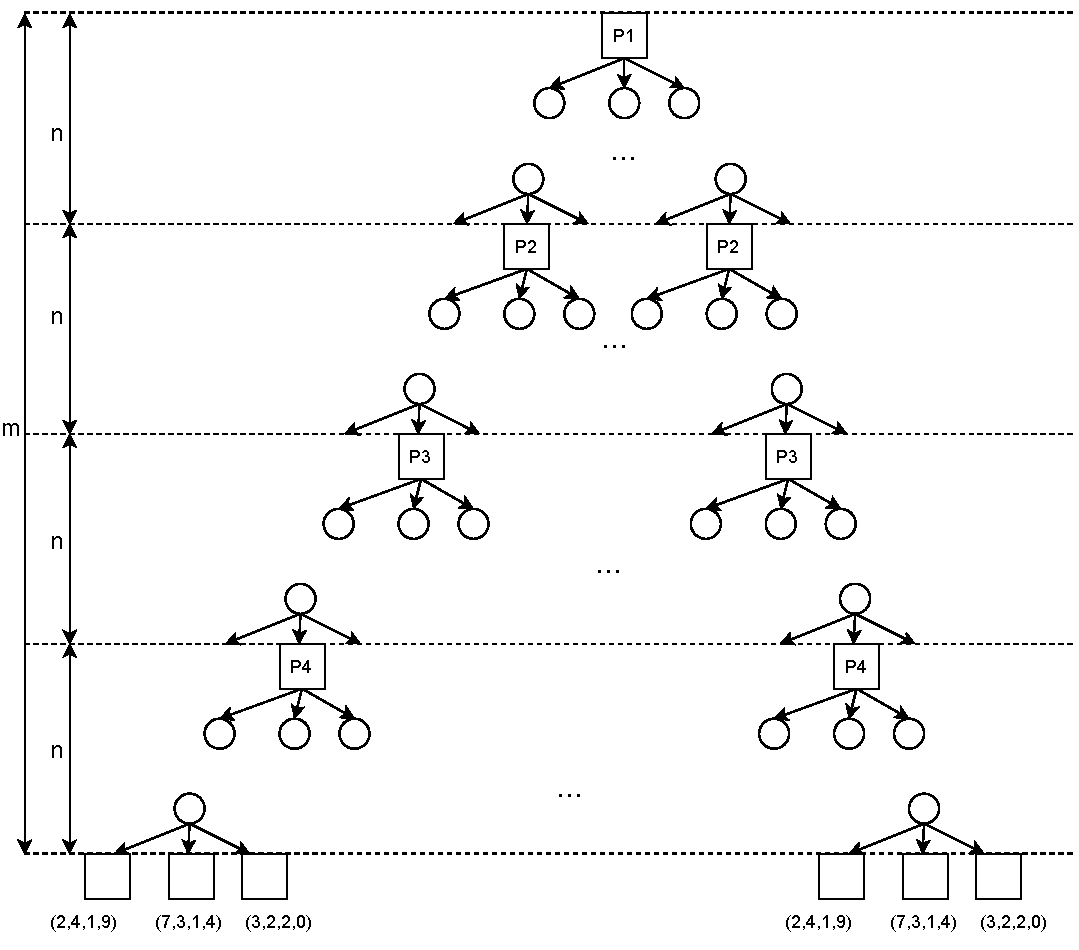
\includegraphics[width=.6\textwidth]{figures/sui-dfs.pdf}
	\caption{Prehľadávanie stavového priestoru pomocou \textit{Max-N}.}
	\label{img:dfs}
\end{figure}

\section{Implementácia prehľadávania}

\subsection{Expandovanie stavu}
Expandovanie uzlu hráča vykoná funkcia \texttt{possible\_moves(board, player)}, ktorá pre aktuálny stav hracej dosky (\texttt{board}) a hráča (\texttt{player}) určí nasledujúce možné ťahy. Možné ťahy sa počítajú podobne ako v botovi STEI. Množina všetkých možných ťahov je ohraničená len na také, ktoré spĺňajú aspoň jedno z nasledujúcich kritérií:
\begin{itemize}
	\item Pravdepodobnosť úspešného útoku na oblasť a súčasne udržanie tejto oblasti v nasledujúcom ťahu je väčšia alebo rovná $\frac{1}{2}$.
	\item Hráč má v útočiacom poli plný počet kociek (8).
\end{itemize}

\subsection{Simulácia ťahu hráča}
Každý expandovaný ťah je simulovaný funkciou \texttt{apply\_move\_to\_board(board, action)}. Simulácia zoberie aktuálny stav hracej dosky (\texttt{board}), navrhovaný ťah (\texttt{action}) a vytvorí nový stav hracej dosky. Útočný ťah je v tejto hre stochastický avšak simulácia je deterministická a uvažuje, že útočník zvíťazí vždy ak má väčšie množstvo kociek ako obranca.

\subsection{Ohodnotenie listového uzlu}
Na ohodnotenie listového uzlu používame metriku, ktorá zohľadňuje najväčší región vlastnený každým hráčom. Región je súvislá časť polí na hracej doske, ktorá patrí jedinému hráčovi. V danom listovom uzle sa nájde najväčší región pre každého hráča a počet oblastí v tomto regióne je ohodnotením skóre pre daného hráča.

\subsection{Konfigurácia parametrov prehľadávania}
Parameter $n$ (hĺbka prehľadávania ťahov v rámci jedného hráča) je nastavená na 1 pretože väčšia hĺbka znižovala pomer výhier nášho AI. 

Parameter $m$ (hĺbka prehľadávania v rámci kôl) je nastavená taktiež na 1. Prehľadávame teda stavový priestor v ktorom každý hráč odohrá jednu sériu svojich ťahov.

\section{Stratégia}
Naše AI funguje podľa stratégie, ktorá je podobná STEI\_ADT. Najsilnejší protihráč je práve bot STEI\_ADT. Preto je naša stratégia podobná jeho. Avšak naša AI ju vylepšuje o prehľadávanie stavového priestoru. Prehľadávanie by malo byť efektívne práve preto, že poznáme implementáciu súperovho bota. Naša simulácia súperovho útočného ťahu teda vychádza zo stratégie STEI, ktorú súper používa. Preto predpokladáme, že vieme pomerne dobre predvídať súperove ťahy. Na druhej strane, hra je pomerne silne stochastická čo simuláciu značne znepresnuje.

Voľba ťahu v každom kole, pričom v jednom kole má hráč viac ťahov, postupuje podľa nasledujúcej stratégie:
\begin{enumerate}
	\item Prvé 4 ťahy AI presunie svoje kocky z vnútra poľa na hranice zo súpermi tak aby malo čo najväčšiu útočnú silu (ofenzíva podobná STEI\_ADT).
	\item AI vykoná prehľadávanie stavového priestoru pomocou \textit{Max-N} a zvolí útočný ťah s najlepším ohodnotením. Tento krok opakuje dokedy mu \textit{Max-N} poskytuje možné útoky. (STEI\_ADT v tejto fáze neprehľadáva stavový priestor ale používa heuristickú funkciu)
	\item Na záver vykoná AI defenzívny presun. Zvyšné 2 ťahy na presun vlastných kociek využije tak aby svoje kocky presunula od hraníc (defenzíva podobná STEI\_ADT).
\end{enumerate}

\section{Umělá inteligence}

Neuronová síť implementuje heuristickou funkci, která se poté využívá k ohodnocení listových uzlů v rámci procedury MaxN. Vstupem neuronové sítě je vektor reprezentující aktuální stav hry, výstupem je potom vektor čtyř reálných čísel z intervalu $\langle 0,1 \rangle$, které udává pravděpodobnost výhry daného hráče v aktuální situaci.

%Neurónová sieť implementuje heuristickú funkciu, ktorá sa potom využíva na ohodnotenie listových uzlov v rámci procedúry MaxN. Vstupom neurónovej siete je vektor reprezentujúci aktuálny stav hry, výstupom je potom vektor štyroch reálnych čísel z intervalu $\langle 0,1 \rangle$, ktoré udáva pravdepodobnosť výhry daného hráča v aktuálnej situácii.

\subsection{Serializace hry}
Pro účely serializace byla upravena serverová část hry, a to konkrétně soubor \texttt{dicewars/server/game.py}. Tato drobná úprava umožňuje uložit všechny stavy her(pole objektů \texttt{board}), které nastávají v rámci jednoho turnaje do souboru \texttt{.pickle}.

Samotná serializace a transformace do HDF\footnote{HDF - Hierarchical Data Format} souboru je implementována skriptem\\\texttt{process\_pickle\_to\_np\_array.py} a probíhá offline (tedy mimo běhové prostředí hry).

Serializovaná hra je reprezentována vektorem čísel o délce $V$, kde celková délka vektoru se vypočte v závislosti na počtu políček následovně: $\frac{bSize}{2} \cdot (1+bSize) + 2 \cdot bSize + 1$. Tento vektor se skládá z celkem tří komponent: 
\begin{itemize}
	\item matice sousednosti $\bm{M}_{n}$ - určuje, zda políčko $i$ sousedí s políčkem $j$. Pokud \textit{$M_{i,j}$} je rovno 1, pak políčko $i$ sousedí s $j$. V případě, že \textit{$M_{i,j}$} je rovno nule, tak nikoliv. Protože je matice symetrická, ukládá se pouze horní trojúhelník (včetně diagonály). Velikost matice sousednosti je určena vztahem: $\frac{bSize}{2} \cdot (1+bSize)$.
	\item vektor vlastnictví $\bm{\vec{o}}$ - reprezentuje informaci o vlastníkovi políčka, vlastník je reprezentován hodnotou z intervalu $\langle 1;4 \rangle$. Velikost vektoru $\bm{\vec{o}}$ je $bSize$.
	\item vektor kostek $\bm{\vec{d}}$ - počet kostek na daném políčku (nabývá hodnot z intervalu $\langle 1;8 \rangle$).  Velikost vektoru $\bm{\vec{d}}$ je $bSize$.
	\item vítěz v rámci současného turnaje - velikost $1$ políčko.
\end{itemize}

\subsection{Neuronová síť}


Generování surových dat probíhalo pomocí následujícího příkazu \texttt{./scripts/dicewars-tournament.py -g 4 -n 1000 --ai-under-test kb.xdolez67} s upraveným serverem (viz předchozí sekce). Tato data byla následně zpracována pomocí skriptu \texttt{process\_pickle\_to\_np\_array.py}, který vytvoří soubor HD5 s numpy polem dimenze (N, 664), kde N je celkový počet stavů her a 664 je velikost jednoho vektoru.

Tento soubor je dále zpracován tak, aby zastoupení výher všech hráču bylo uniformní a zároveň se sníží velikost v první dimenzi a provede se operace shuffle podle první dimenze. Toto zpracování provádí skript \texttt{extract\_subset\_fromH5.py}

Takto zpracovaný soubor je poté vstupem pro skript \texttt{./scripts/network.py}, který data rozdělí na trénovací, testovací a validační a na těchto datech natrénuje neuronovou síť. Architektura neuronové sítě byla zvolena na základě výsledků experimentů.



\section{Záver}


\end{document}
